\chapter{Génération d'un automate}

\paragraph{}
Nous avons vu précédemment que JDart produit un arbre des contraintes. Nous 
allons voir plus en détail dans ce chapitre comment nous pouvons faire pour 
générer un automate de notre applet à partir de l'arbre des contraintes obtenu.

\paragraph{Note technique}
Nous présenterons dans ce chapitre des sorties brutes de JDart car elles
permettent de mieux illustrer nos propos. Toutefois JDart est capable de 
générer une sortie au format JSON. Ce format garde les propriétés qui seront 
présentées ici.

\begin{figure}[H]
 \centering
 \begin{verbatim}
 {
        decision: "(i <= 2000)",
        children: [
                { result: "OK"},
                { 
                        decision: "b",
                        children: [
                                 { result: "OK"}
                                 { result: "ERROR" }
                        ]
                }
        ]
 }
 \end{verbatim}
 \caption{Exemple de fichier JSON généré par JDart}
\end{figure}
C'est ce format que nous utiliserons lors du développement de notre solution 
car il est plus facile à traiter.


\section{Analyse de la sortie}

\paragraph{}
L'arbre des contraintes de JDart suit un schéma simple : une décision conduit 
vers une autre décision ou vers un état terminal, en fonction de la valeur de 
la décision.
\par
Une décision s'effectue sur la valeur d'une variable, elle correspond à une 
instruction conditionnel dans le code (\textbf{if/else}, \textbf{switch}) ou à 
une boucle (\textbf{while}, \textbf{for}). Nous allons présenter comment JDart 
représente ces instructions.

\paragraph{Condition if/else}
Une condition est l'évaluation d'une variable ou expression booléenne qui mène 
à deux états différents du programme. La sortie de JDart se compose de 
l'expression à vérifier, suivit d'une instruction si la condition est vrai 
puis d'une autre instruction dans le cas où elle ne l'est pas :

\begin{verbatim}
Si i != 1
   instruction si vrai
   instruction si faux
\end{verbatim}

\paragraph{}
Une instruction peut être une nouvelle condition ou un état final.

\paragraph{Table switch}
Les instructions \textbf{switch} peuvent être transformé en une imbrication de 
\textbf{if/else}, où chaque \textbf{if} correspond à un \textbf{case} :

\begin{minted}{java}
 switch(i) {
 case 1:
	// code cas 1
	break;
 case 2:
	// code cas 2
	break;
 // ...
 default:
	code cas défaut
 }
\end{minted}

peut être écrit :
\begin{minted}{java}
 if(i == 1) {
	// code cas 1
 } else {
	if(i == 2) {
		// code cas 2
	} else {
		// code cas défaut
	}
 }
\end{minted}

De la même manière pour JDart, les \textbf{switch} sont une succession de 
décisions.

\paragraph{Boucle for,while}
Pour gérer le cas des boucles, JDart tente de lister les valeurs générées par 
les différentes itérations et d'imbriquer les décisions  qu'il en résulte.


Par exemple pour le code suivant :

\begin{minted}{java}
for (int j = 1; j < 4; j++) {
      if (i + j > 0) {
      	System.out.println((i + j) + " is > 0");
      } else {
      	System.out.println((i + j) + " is <= 0");
      }
}
\end{minted}
on obtient la sortie :
\begin{figure}[H]
 \centering
 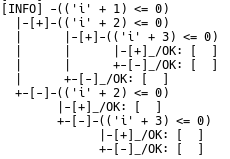
\includegraphics[]{./images/jdart_loops.png}
 \caption{Sortie JDart d'une boucle for}
\end{figure}

Ici JDart énumère toutes les valeurs de $j$ allant de 1 à 4 et "embo\^ite" les 
condition de (if/else), nous obtenons alors une version linéaire de la boucle 
for.

Nous obtenons le même comportement avec une boucle while.

\paragraph{État final}
Un état final est une instruction dans le code qui permet à JDart d'arrêter son 
exploration dans une branche, il existe de type d'état final : 
\begin{itemize}
 \item les cas d'erreurs : cela correspond le plus souvent à une exception 
levée et/ou non attrapée.
 \item les cas valides : c'est-à-dire une instruction ou une suite 
d'instructions ne contenant aucune décision à prendre et où aucune erreur n'est 
levée. Un cas valide peut ne correspondre à aucune instruction dans le code 
source, seulement on explicite toutes les branche du code.

\begin{figure}[H]
	\centering	
	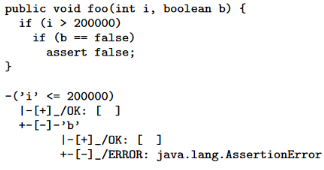
\includegraphics[scale=0.5]{images/jdart_exemple.png}
	\caption{\label{fig:jdart_sample} Exemple de sortie JDart}
	\label{fig:exemple_out_jdart}
\end{figure}

Dans cet exemple les deux états "OK" ne corresponde à aucune instruction dans 
le code, seulement dans les deux cas aucune erreur n'est levée et la fonction 
prend fin.

\end{itemize}

\paragraph{}
Nous pouvons maintenant dire que l'arbre des contraintes est en réalité un 
arbre binaire suivant un schéma simple :
\begin{verbatim}
Condition
        Instruction si Contidion vraie
        Instruction si Condition fausse
\end{verbatim}



\section{Construire un graphe}

\paragraph{}
Maintenant que nous comprenons mieux la structure des données que génère JDart 
nous pouvons construire l'automate qui en résulte. Nous allons ici présenter un 
algorithme qui permettra de construire un automates à partir d'un arbre des 
contraintes puis nous l'appliquerons à un exemple.

\subsection{Algorithme}

\paragraph{}
Pour rappel un automate se compose d'une liste d'états et de transitions qui 
permettent d'évoluer d'un état à un autre, il y a également un état initial 
et une liste d'états finaux.


Pour construire notre automate nous devons d'abord ajouter un état initial qui 
correspond à l'entrée du programme ou de la fonction analysée. Les états finaux 
sont le cas valide et les cas d'erreur, on pourra ajouté plusieurs états 
d'erreur en fonction des exception levé.

\paragraph{}
Pour la suite nous utiliserons la structure de données suivante pour 
représenter un automate :

$$A = ( E, q, F, \delta )$$
où $E$ est la liste des états, $q$ l'état initial, $F$ la liste des états 
finaux 
et $\delta$ la liste des transition. Nous représenterons les transition de la 
manière suivante : $(etatDepart, etiquette, etatArrive)$.

\paragraph{}
Les noeuds de l'arbre des contraintes seront définit tel que :
$$ N = (decision, enfantVrai, enfantFaux)$$


L'algorithme consiste à parcourir en profondeur l'arbre entièrement.
Cela donne l'algorithme récursif suivant :

\newpage
\begin{verbatim}
Fonction ConstruireAutomate(ArbreContrainte arbre, Noeud n = noeud racine de 
l'arbre, Etat e = q l'état initial)
Début
        A : Automate
	
        Si e est un etat final de A
                Retourner 
        Fin Si
        
        Si n.enfantVrai est un état final ET n.enfantVrai n'est pas dans A
                nouvelEtat = A.ajouterEtatFinal(n.enfantVrai)
        Sinon Si n.enfantVrai est un état final de A
                nouvelEtat = A.obtenirEtatCorrespondant(n.enfantVrai)
        Sinon
                nouvelEtat = A.ajouterEtat(n.enfantVrai)
        Fin Si
	
        A.ajouterTransition(e, n.decision, nouvelEtat)
        ConstruireAutomate(arbre, n.enfantVrai, nouvelEtat)

        Si n.enfantFaux est un état final ET n.enfantFaux n'est pas dans A
                nouvelEtat = A.ajouterEtatFinal(n.enfantFaux)
        Sinon Si n.enfantFaux est un état final
                nouvelEtat = A.obtenirEtatCorrespondant(n.enfantFaux)
        Sinon
                nouvelEtat = A.ajouterEtat(n.enfantFaux)
        Fin Si
	
        A.ajouterTransition(e, Iverser(n.decision), nouvelEtat)
        ConstruireAutomate(arbre, n.enfantFaux, nouvelEtat)
Fin
\end{verbatim}

\paragraph{}
La fonction \textbf{Inverser()} retourne l'expression booléenne inverse, par 
exemple pour $i == 10$ elle retourne $i \ne 10$. 

\subsection{Exemple d'exécution}

Pour exécuter cet algorithme nous allons reprendre l'exemple de la Figure 
\ref{fig:exemple_out_jdart}. L'algorithme commence avec un automate ne 
contenant que l'état initial :

\begin{figure}[H]
 \centering
 \includegraphics[scale=.46]{./images/graph_build.png}
 \caption{Automate au début de l'algorithme}
\end{figure}


 
 \begin{figure}[H]
  \centering
  \includegraphics[scale=0.46]{./images/graph_build_1.png}
  \caption{Étape 1 : Exploration de l'arbre (profondeur 1)}
 \end{figure}

 \paragraph{} On explore le côté "vrai" de l'arbre des contraintes, nous 
arrivons sur une état final, qui est 
ajouté à l'automate ainsi que la transition pour y arriver. Au deuxième appel, 
l'exploration de ce côte de l'arbre s'arrête et passe à l'autre côté.


 \begin{figure}[H]
  \centering
  \includegraphics[scale=0.46]{./images/graph_build_2.png}
  \caption{Étape 2 : Exploration de l'arbre (profondeur 1)}
 \end{figure}
 \paragraph{} Ici le nouvel état n'est pas un état final, il faut continuer 
l'exploration.
 \paragraph{} Et ainsi de suite jusqu'à ce que l'arbre soit 
entièrement exploré.


 \begin{figure}[H]
  \centering
  \includegraphics[scale=0.46]{./images/graph_build_3.png}
  \caption{Étape 3 : Exploration de l'arbre (profondeur 2)}
 \end{figure}

\begin{figure}[H]
  \centering
  \includegraphics[scale=0.46]{./images/graph_build_4.png}
  \caption{Étape 4 : Exploration de l'arbre (profondeur 2)}
 \end{figure}


\paragraph{}
À la fin de l'algorithme nous obtenons bien un automate correspondant à 
l'exécution de ce code. Il alors possible d'en déduire les valeurs de $i$ et 
$b$ qui permettent d'aboutir à un état valide ou d'erreur.


\begin{comment}




\chapter{Soot}

\paragraph{}
Dans ce chapitre nous allons présenter \cite{Soot} qui est un outils permettant 
de la compilation et l'analyse du code source.

	\section{Présentation de Soot}

	\paragraph{}
	À l'origine Soot est un framework qui à pour but d'optimiser du code. 
Soot a été produit par le groupe de recherche Sable de l'université de McGill. 
Concrètement ce framework permet de :

	\begin{itemize}
		\item analyser points par points
		\item créer des graphes de séquence
		\item créer des graphes de flux de contrôle
		\item instrumenter du code
	\end{itemize}

	\paragraph{}
	Soot propose plusieurs représentations intermédiaires du code. Chaque 
représentation intermédiaire correspond à un niveau d'abstraction.

	\paragraph{Baf} est une représentation simplifiée du bytecode Java. Il 
permet de manipuler du bytecode plus simplement.
	\paragraph{Jimple} est la représentation principale de Soot. C'est une 
représentation à trois adresses, c'est-à-dire qu'une instruction peut contenir 
trois variables. Par exemple l'instruction suivante : 
	$$ a = (b + 1) * c - d$$
	Devient : 
	$$ \$i_0 = b + 1$$
	$$ \$i_1 = \$i_0 * c$$
	$$ a = \$i_1 - d$$
	où \$i0 et \$i1 sont des variables intermédiaires.


	Le jeu d'instructions est aussi réduit (15 instructions contre plus de 
200 en bytecode).
	\paragraph{Shimple} est une représentation de type \gls{SSA}, c'est une 
représentation qui interdit la réaffectation d'une variable, des versions de 
variables sont utilisées pour remplir ce critère. Par exemple le code suivant :
	$$ y = 1 $$
	$$ y = 2 $$
	$$ x = y $$
	Devient :
	$$ y_1 = 1 $$
	$$ y_2 = 2 $$
	$$ x_1 = y_2 $$ 
	Cela permet de voir que la première instruction est inutile. Shimple 
permet donc d'éliminer du code mort, de contrôler la propagation de constante...

	\paragraph{Grimp} est une représentation basé sur Jimple, elle 
n'utilise pas de variable intermédiaire ce qui la rapproche plus du langage 
Java. Elle est utilisée pour de la décomplilation ou pour de l'inspection de 
code.

\section{}

\paragraph{}
\end{comment}
